\section{Experimentos e resultados}

Os experimentos usam a série mensal canônica de TDS (182 meses, fevereiro de 2011 a março de 2026), sem valores ausentes.

\subsection{Tendência bruta e reenquadramento cíclico}

Cinco métodos com ajuste global à série inteira (Mann-Kendall/Sen, Theil-Sen, OLS, STL+tendência, regressão bayesiana) convergem para uma tendência de alta estatisticamente significativa, entre 2,9 e 3,9~mg/L/ano (p$<$0,01 em todos os casos), com previsões de +20 anos entre 774 e 807~mg/L (Figura \ref{fig:tendencia-tds}). Esse resultado, porém, \textbf{não é robusto} a duas escolhas metodológicas: restrita ao período pós-2012 (\texttt{EFF-001A}, 170 dos 182 meses), a inclinação cai para 0,84~mg/L/ano e deixa de ser significativa (p=0,59); e a significância do teste de Mann-Kendall se inverte conforme a correção de autocorrelação adotada (significativa sob a correção padrão e sob \textit{trend-free pre-whitening}; não significativa sob \textit{pre-whitening} simples e sob a correção de Hamed-Rao).

\begin{figure}[H]
    \centering
    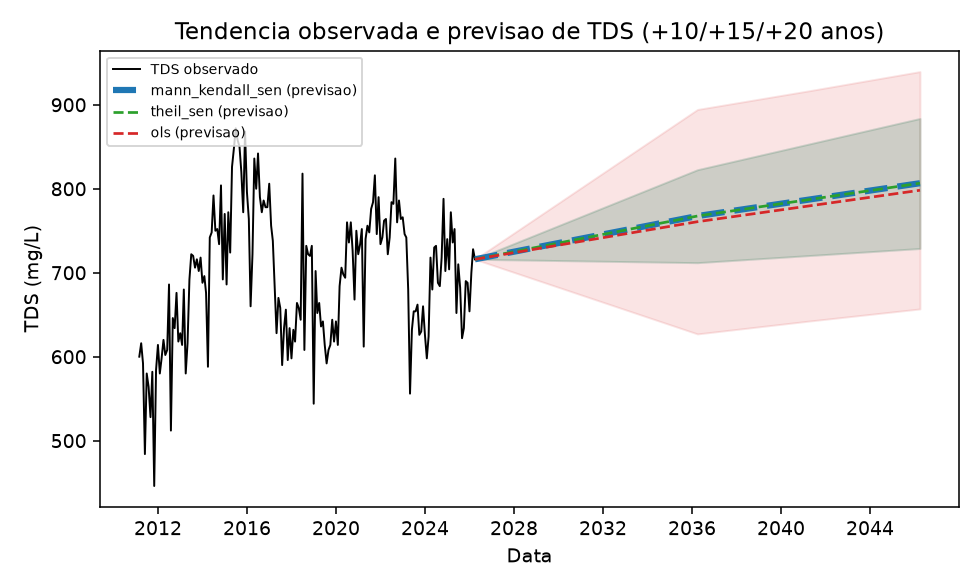
\includegraphics[width=0.9\linewidth]{images/tendencia-tds.png}
    \caption{TDS observado (2011--2026) e previsão de tendência, com incerteza para +10/+15/+20 anos.}
    \label{fig:tendencia-tds}
\end{figure}

Investigando essa fragilidade, uma hipótese de degrau artificial na transição de código de monitoramento (\texttt{EFF-001}$\to$\texttt{EFF-001A}, $\sim$2012) foi testada e \textbf{rejeitada}: a transição é contínua mês a mês, mesmo método analítico, mesmas coordenadas. Em vez disso, a série revelou um \textbf{padrão cíclico por regime}: alta de 563 para 808~mg/L entre 2011 e 2015 (coincidindo com a seca da Califórnia de 2012--2016), queda até 636~mg/L em 2019, nova alta até 768~mg/L em 2022 (segunda seca, 2020--2022) e leve recuo depois.

\subsection{PDSI confirma o padrão cíclico}

Para testar essa hipótese com uma variável externa, a série foi cruzada com o Índice de Severidade de Seca de Palmer (PDSI) mensal do NOAA (Figura \ref{fig:pdsi-regimes}). A correlação bruta é forte e altamente significativa mesmo após corrigir o número efetivo de observações independentes (Califórnia estadual: $r=-0{,}651$, p=0,0003, defasagem de 4 meses); \textit{changepoints} detectados de forma independente no PDSI (sem informar as datas do TDS ao algoritmo) coincidem com as quatro viradas de regime observadas (2012, 2015, 2019, 2022) dentro de poucos meses; e uma decomposição de importância relativa (LMG, $\mathrm{TDS} \sim \mathrm{PDSI}_{\text{defasado}} + \mathrm{vazao}$) atribui 68 a 79\% da importância ao PDSI nas três séries testadas -- mesma ordem de grandeza do benchmark de um estudo independente com 26 estações da região (~88\% água de origem, \cite{scsc2018tds}). A correlação sobre séries destendenciadas é mais fraca e muda de sinal, indicando que a seca explica principalmente o nível médio de cada regime, não a oscilação mês a mês fina.

\begin{figure}[H]
    \centering
    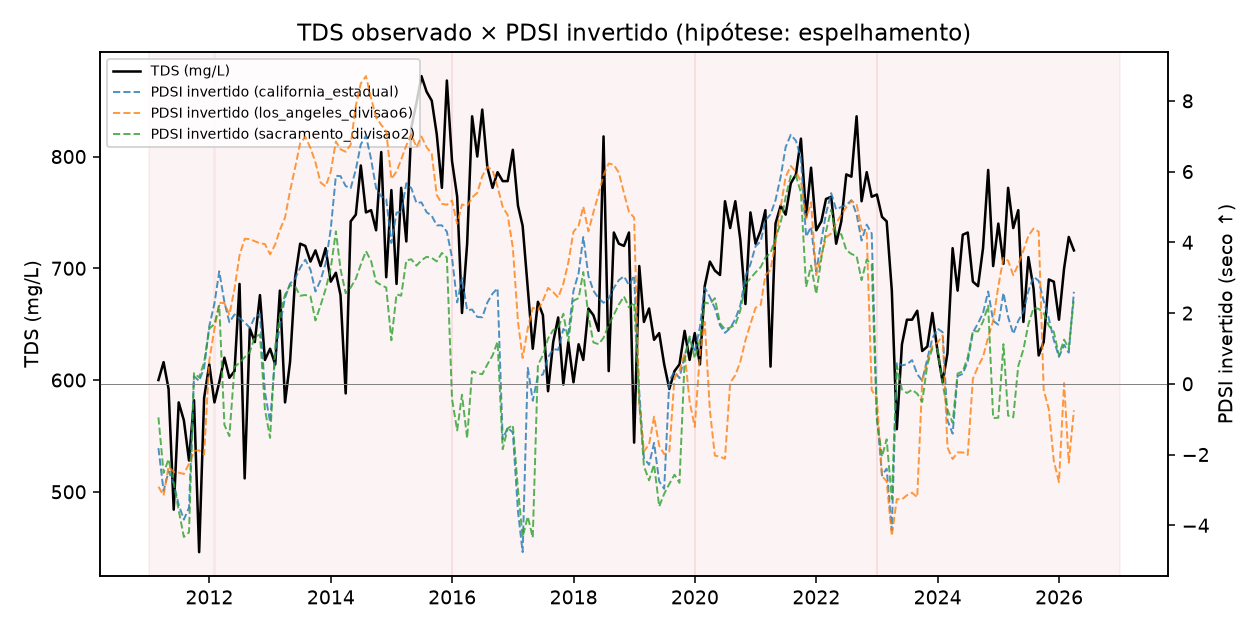
\includegraphics[width=0.95\linewidth]{images/pdsi-vs-tds-regimes.png}
    \caption{TDS observado × PDSI invertido, com os regimes identificados sombreados.}
    \label{fig:pdsi-regimes}
\end{figure}

\subsection{Mecanismo causal: diluição, não mais sal}

O WRTDS (normalização por vazão) mostra que a tendência bruta de $\log(\mathrm{TDS})$ (+0,582\%/ano, p=0,0056) \textbf{quase desaparece} após descontar o efeito da vazão (-0,133\%/ano, p=0,064, não significativa) -- resultado confirmado por checagem de circularidade (vazão derivada de Cloreto, independente do TDS). O balanço de massa (Figura \ref{fig:balanco-massa}) confirma essa leitura diretamente: a carga de sal caiu $-3{,}20\%$/ano e a vazão caiu $-3{,}85\%$/ano no mesmo período (p$<$0,0001 em ambos) -- \textbf{o mecanismo é diluição, não mais sal entrando no sistema} (validação histórica: RMSE=19,1~mg/L, $r=0{,}973$). A extrapolação linear desses componentes por 20 anos cruza valores fisicamente implausíveis (vazão negativa em +20 anos), motivando a projeção por cenários da próxima seção em vez de uma previsão pontual.

\begin{figure}[H]
    \centering
    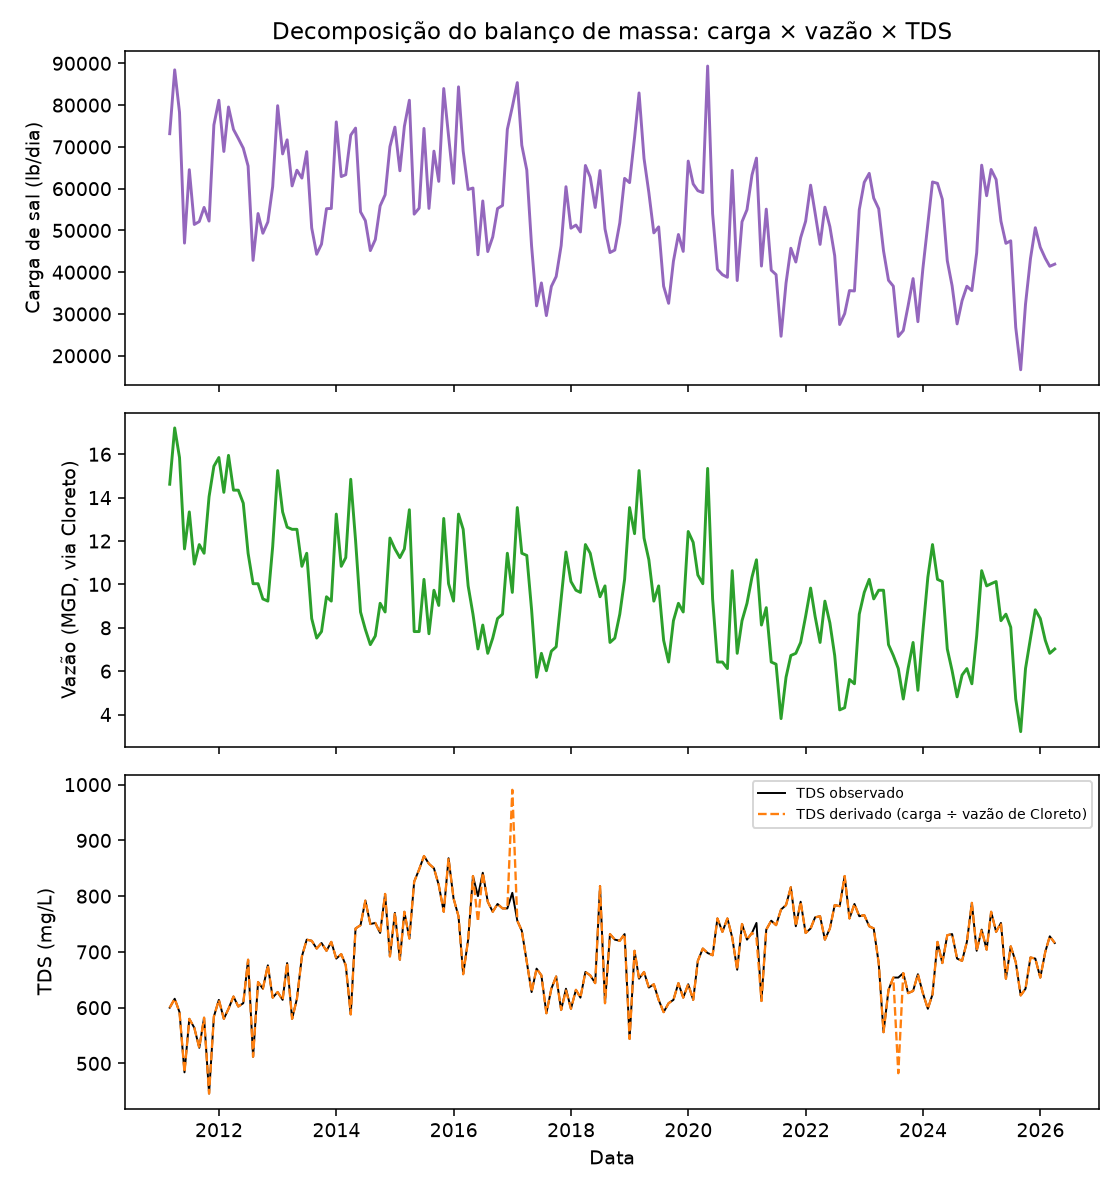
\includegraphics[width=0.95\linewidth]{images/balanco-massa-decomposicao.png}
    \caption{Decomposição do balanço de massa: carga de sal, vazão e TDS derivado vs.\ observado.}
    \label{fig:balanco-massa}
\end{figure}

\subsection{Previsão: cenários climáticos e finalistas da bateria}

Em vez de um valor único, a previsão de longo prazo é uma faixa condicionada a cenários de seca, via simulação de Monte Carlo sobre o PDSI histórico (Tabela \ref{tab:cenarios}, Figura \ref{fig:cenarios}). Todas as faixas são fisicamente plausíveis, ao contrário da extrapolação linear.

\end{multicols*}
\begin{table}[H]
    \centering
    \begin{tabular}{l|c|c|c}
         Cenário & +10 anos & +15 anos & +20 anos \\ \hline
        Seco & 721 [596, 852] & 720 [595, 848] & 718 [588, 846] \\
        Agravamento climático & 682 [561, 808] & 697 [576, 826] & 714 [591, 842] \\
        Normal & 663 [536, 788] & 659 [533, 784] & 658 [529, 783] \\
        Úmido & 597 [470, 721] & 595 [470, 723] & 594 [462, 721] \\
    \end{tabular}
    \caption{Mediana [P5, P95] de TDS simulado (mg/L) por cenário climático e horizonte.}
    \label{tab:cenarios}
\end{table}
\begin{multicols*}{2}

\begin{figure}[H]
    \centering
    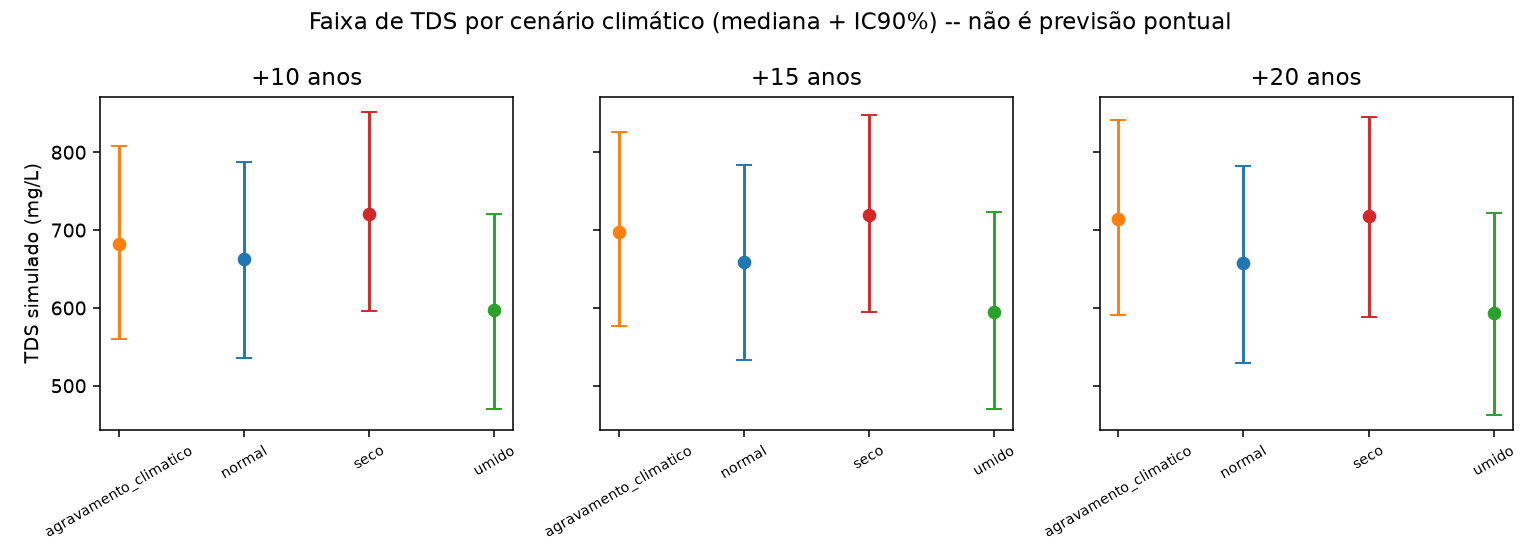
\includegraphics[width=0.95\linewidth]{images/cenarios-pdsi-horizontes.png}
    \caption{Faixa de TDS por cenário climático e horizonte (mediana + IC90\%).}
    \label{fig:cenarios}
\end{figure}

Paralelamente, dos 35 métodos da bateria original, três finalistas foram recomendados por representarem mecanismos de extrapolação distintos e pelo melhor desempenho combinado (MASE, diagnóstico de resíduos, comportamento do IC): regressão bayesiana (única com incerteza genuinamente crescente por construção), Detrend+RF (melhor MASE entre os métodos sem saturar, único sem autocorrelação residual detectável NO AJUSTE IN-SAMPLE -- o mesmo teste sobre o resíduo de \textit{holdout} já não distingue Detrend+RF dos demais; sua vantagem de erro sobre sarima/híbrido, porém, é estatisticamente real (Diebold-Mariano, p$<$0,05)) e híbrido SARIMA+Prophet (melhor RMSE entre os métodos de série temporal). Os três convergem para um intervalo relativamente estreito de pontos centrais (Tabela \ref{tab:finalistas}, Figura \ref{fig:finalistas}) -- acima da faixa condicionada a cenários, porque a extrapolação de tendência bruta carrega implicitamente o pressuposto de que a vazão continua caindo livremente, ao passo que os cenários limitam a vazão futura a valores historicamente plausíveis. A cobertura empírica do IC90 desses finalistas (teste de robustez \url{script_31_testes_robustez_avancados.py}), porém, só se aproxima do nominal de 90\% para a regressão bayesiana (86,7\% via CV expansiva); híbrido SARIMA+Prophet e Detrend+RF ficam em 75,0\% e 26,7\% -- os IC90 desses dois, e dos horizontes de +10/+15/+20 anos em geral, devem ser lidos como ilustrativos da ordem de grandeza, não como intervalos estatisticamente calibrados.

\end{multicols*}
\begin{table}[H]
    \centering
    \begin{tabular}{l|c|c|c}
         & +10 anos & +15 anos & +20 anos \\ \hline
        Regressão bayesiana & 758,2 [624,2; 893,1] & 778,7 [636,4; 917,2] & 797,7 [658,1; 937,8] \\
        Detrend + RF & 743,5 [641,0; 845,9] & 762,2 [636,7; 887,7] & 780,9 [636,0; 925,8] \\
        Híbrido SARIMA+Prophet & 714,4 [130,1; 1501,5] & 738,9 [-94,3; 1832,3] & 763,5 [-332,3; 2176,6] \\
    \end{tabular}
    \caption{Previsão pontual e IC90\% (mg/L) dos três finalistas.}
    \label{tab:finalistas}
\end{table}
\begin{multicols*}{2}

\begin{figure}[H]
    \centering
    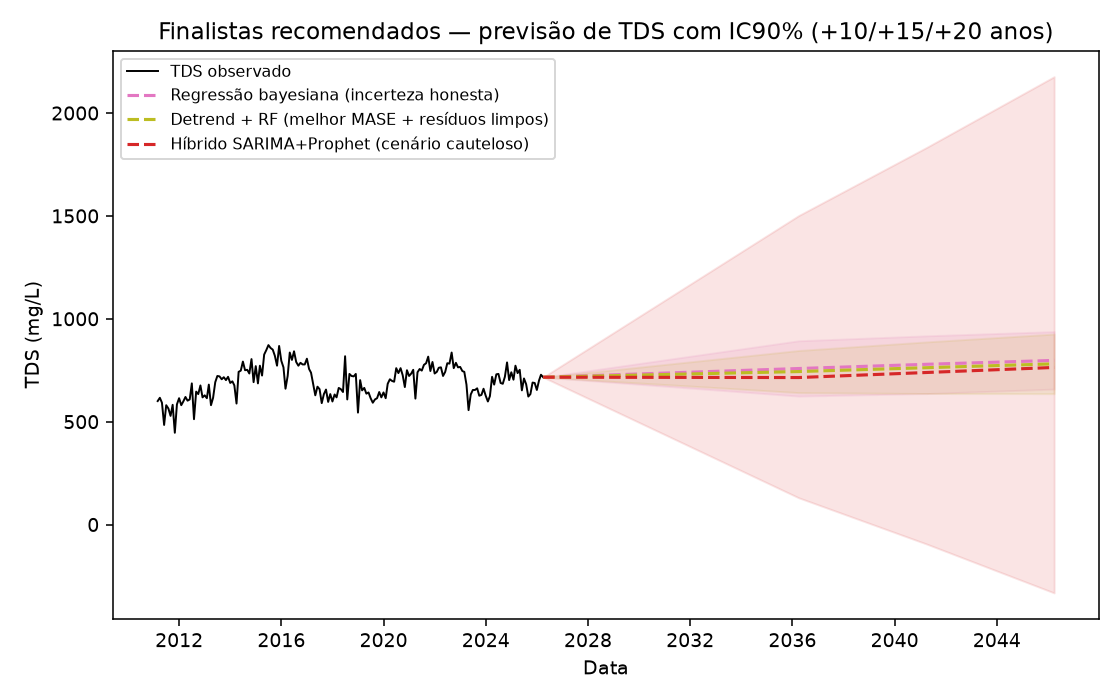
\includegraphics[width=0.95\linewidth]{images/sintese-final-finalistas.png}
    \caption{Finalistas recomendados, com IC90\% para +10/+15/+20 anos.}
    \label{fig:finalistas}
\end{figure}

\subsection{Correlação com desempenho biológico}

TDS correlaciona-se positivamente com Amônia mesmo após remover a tendência comum de ambas as séries ($r=0{,}175$, p=0,018; mais forte com 1 mês de defasagem, $r=0{,}215$) -- meses de salinidade acima do esperado coincidem com nitrificação pior que o esperado, dando plausibilidade biológica à preocupação original que motivou este trabalho. Já TDS vs.\ BOD é \textbf{negativo e não significativo} nos três tratamentos de dado censurado testados ($r$ entre $-0{,}068$ e $-0{,}126$, p entre 0,090 e 0,360) -- o oposto da hipótese inicial; a leitura mais provável é falta de variação real na série de BOD, que permanece rente ao limite de detecção durante quase todo o período (Figura \ref{fig:correlacao}).

\begin{figure}[H]
    \centering
    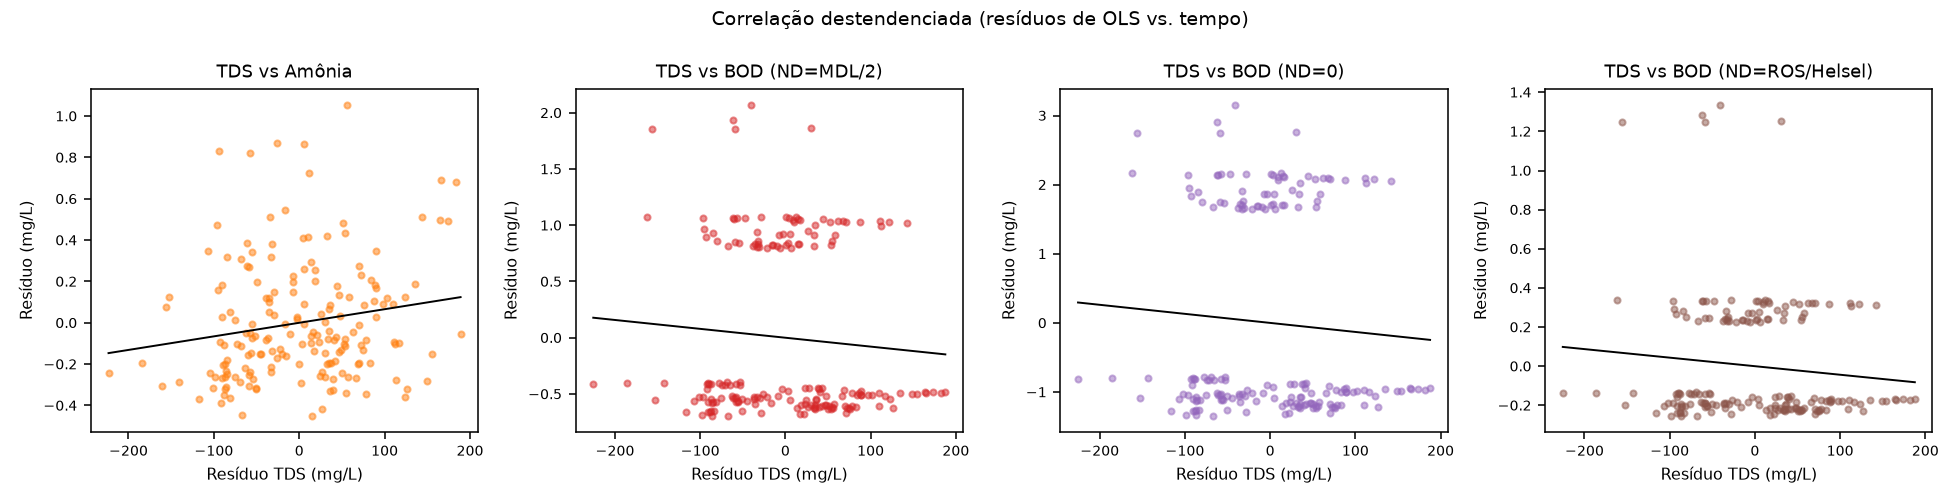
\includegraphics[width=\linewidth]{images/correlacao-tds-amonia-bod.png}
    \caption{Correlação entre os resíduos (após remoção da tendência) de TDS e de Amônia/BOD.}
    \label{fig:correlacao}
\end{figure}

\subsection{Achados complementares}

Re-treinar os 12 métodos que aceitam regressor exógeno com o PDSI como covariável não produziu melhora consistente (só 4 de 12 melhoraram o RMSE de \textit{holdout}); testes adicionais de representação (múltiplos \textit{lags}, seleção por validação cruzada) confirmaram que só o XGBoost tinha margem real de ganho (-5,3\% no \textit{holdout}, -2,0\% na CV). Separadamente, uma série de TDS de origem construída a partir de 21 relatórios anuais da LADWP (2004--2024, auditados célula a célula) correlaciona com o TDS de efluente em $r=0{,}912$ (p=0,000005) -- mais forte que a correlação com o PDSI, e a evidência mais direta obtida neste trabalho de que a qualidade da água de origem é o principal determinante do TDS de efluente.
